\documentclass[a4paper]{article}
\usepackage[utf8]{inputenc}
\usepackage[T1]{fontenc}
\usepackage[french]{babel}
\usepackage{amsmath,amsfonts,amssymb}
\usepackage{bookman}
\usepackage{xcolor}
\usepackage{array}
\usepackage{pifont}
\usepackage{ulem}
\usepackage{listings}
\usepackage{graphicx}
\usepackage{eurosym}
\usepackage{hyperref}
\usepackage[left=2cm, right=2cm, top=2cm, bottom=2cm]{geometry}
\frenchbsetup{StandardLists=true}
\newcommand\coord[3]{\begin{pmatrix}
#1 \\
#2 \\
#3
\end{pmatrix}}
\newcommand{\R}{\mathbb{R}}
\newcommand{\N}{\mathbb{N}}
\newcommand{\D}{\mathbb{D}}
\newcommand{\Z}{\mathbb{Z}}
\newcommand{\Q}{\mathbb{Q}}
\newcommand{\C}{\mathbb{C}}
\newcommand{\K}{\mathbb{K}}
\newcommand{\lra}{\Longrightarrow}
\newcommand{\lla}{\Longleftarrow}
\newcommand{\llra}{\Longleftrightarrow}
\setlength{\textheight}{23.5cm}
\newcommand{\ra}{\rightarrow}
\newcommand{\la}{\leftarrow}

\let\oldsection\section{}
\renewcommand{\section}[1]{\textcolor{purple}{\oldsection{#1}}}
\let\oldsubsection\subsection{}
\renewcommand{\subsection}[1]{\textcolor{cyan}{\oldsubsection{#1}}}
\let\oldsubsubsection\subsubsection{}
\renewcommand{\subsubsection}[1]{\textcolor{orange}{\oldsubsubsection{#1}}}
\let\oldtextbf\textbf
\renewcommand{\textbf}[1]{\textcolor{orange}{\oldtextbf{#1}}}
\let\oldunderline\underline{}
\renewcommand{\underline}[1]{\textcolor{purple}{\oldunderline{#1}}}
\let\oldtextit\textit
\renewcommand{\textit}[1]{\textcolor{violet}{\oldtextit{#1}}}

\lstset{inputencoding=utf8,
        extendedchars=true,
        literate=%
        {é}{{\'{e}}}1
        {è}{{\`{e}}}1
        {ê}{{\^{e}}}1
        {ë}{{\¨{e}}}1
        {û}{{\^{u}}}1
        {ù}{{\`{u}}}1
        {â}{{\^{a}}}1
        {à}{{\`{a}}}1
        {î}{{\\^{i}}}1
        {ô}{{\^{o}}}1
        {ç}{{\c{c}}}1
        {Ç}{{\c{C}}}1
        {É}{{\'{E}}}1
        {Ê}{{\^{E}}}1
        {À}{{\`{A}}}1
        {Â}{{\^{A}}}1
        {Î}{{\^{I}}}1,
        basicstyle=\footnotesize\sffamily\color{black},
        commentstyle=\textcolor{gray},
        numbers=left,
        numbersep=5pt,
        numberstyle=\textcolor{gray},
        keywordstyle=\textcolor{teal},
        showspaces=false,
        showstringspaces=false,
        stringstyle=\textcolor{magenta},
        tabsize=2
}

\title{Rapport du projet de réseau}
\author{Danyl El-Kabir et François Grabenstaetter}

\begin{document}
\sffamily
\everymath{\displaystyle}
\setlength\parindent{0mm}
\setlength{\parskip}{0.2cm}
\maketitle

\begin{center}
    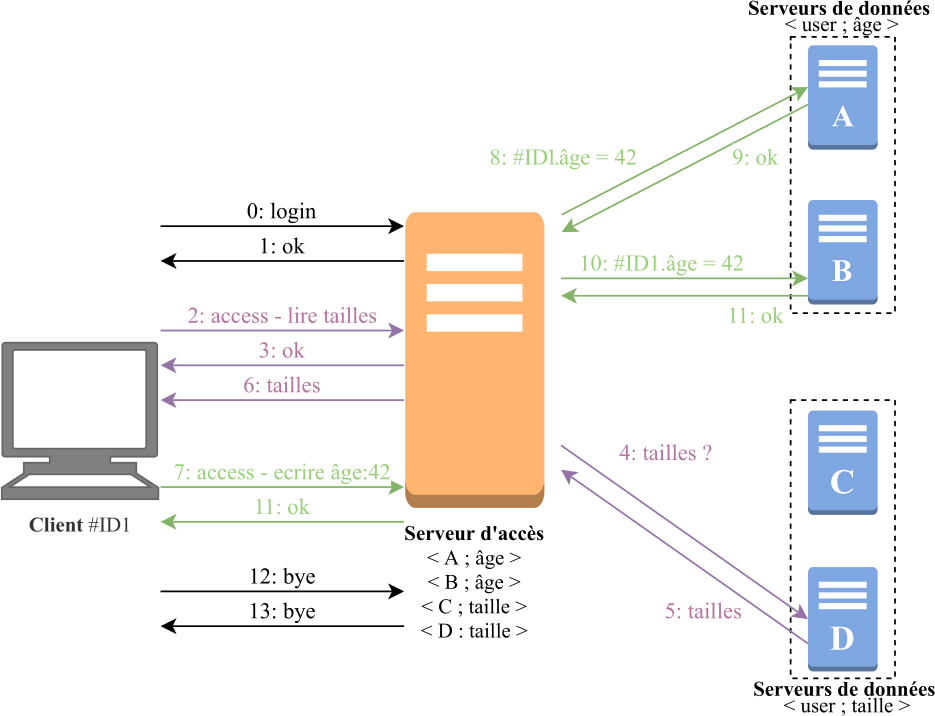
\includegraphics[scale=1.6]{img/enonce.png}
\end{center}

\section{Architecture de la banque de données}

L'architecture de notre projet contient \textbf{4 modules}:
\begin{itemize}
    \item Le \textit{serveur d'accès} (relais)
    \item Le \textit{client}
    \item Le \textit{serveur de données} (nœud)
    \item Les \textit{outils} réseau partagés (common)
\end{itemize}

Nous avons rendu possible la communication de multiples clients en parallèle avec le serveur d'accès ainsi que celle des serveurs de données avec le serveur d'accès.

\subsection{Le serveur d'accès}

Le serveur d'accès \textbf{stocke une liste}:
\begin{itemize}
    \item Des \textit{infos clients} (login, mot de passe et champs autorisés en lecture).

    \item Des \textit{clients connectés} (uniquement ceux dont l'authentification a réussie). On stocke leurs \underline{coordonnées} (IP + port), leur \underline{login}, et la \underline{date} (timestamp) de leur dernier message (déconnexion forcée après \textbf{timeout}).

    \item Des \textit{serveurs de données connectés}. On stocke leurs \underline{coordonnées} (IP + port), le \underline{champ} qu'ils déservent (âge, taille, etc.), un \underline{identifiant} unique qui leur est attribué (utile pour faire correspondre un message reçu avec un serveur de données), la \underline{date} (timestamp) de dernière communication avec ce dernier (retiré de force après \textbf{timeout}), ainsi qu'un booléan \underline{active} pour savoir si le serveur de données est en capacité de traiter des requêtes ou non.

    Par exemple, un serveur de données est \textit{inactif} (active == false) lorsqu'il vient de se connecter et qu'il y a déjà \textbf{un serveur de données de même champ} connecté, le temps que ce serveur de données déjà connecté lui transmet ses données (requêtes SYNC + GETDATA).

    \item Des \textit{réponses en attente}. Il s'agit de faire correspondre une requête \textit{Serveur d'accès $\ra$ Serveur\underline{s} de données} avec les réponses à cette requête afin de n'envoyer qu'une seule et unique réponse au client l'ayant engendré en fonction des réponses / non réponses des serveurs de données interrogés (pour les requêtes \textit{écriture} et \textit{suppression}).

    On stocke un \underline{identifiant} unique pour la structure de réponses en attente, le \underline{client connecté} ayant engendré la requête (et qui devra recevoir la réponse), le \underline{nombre de requêtes envoyées} ainsi que le \underline{nombre de requêtes reçues}, le \underline{type de requête} associé (écriture ou suppression) ainsi que la \underline{date} (timestamp) de création de la structure (envoi d'une réponse forcée après \textbf{timeout}).
\end{itemize}

Les \textbf{timeout} ($\theta$) associés aux clients et aux serveurs de données sont déclenchés après un certain temps $\phi$, mais il y a d'abord \textit{envois successifs} de messages \textbf{PING} durant un interval de temps $\mu$, de sorte que: $\phi = \lambda + k\mu$, avec $\lambda, k\in \N$.

\newpage
\subsection{Le client}

\begin{center}
    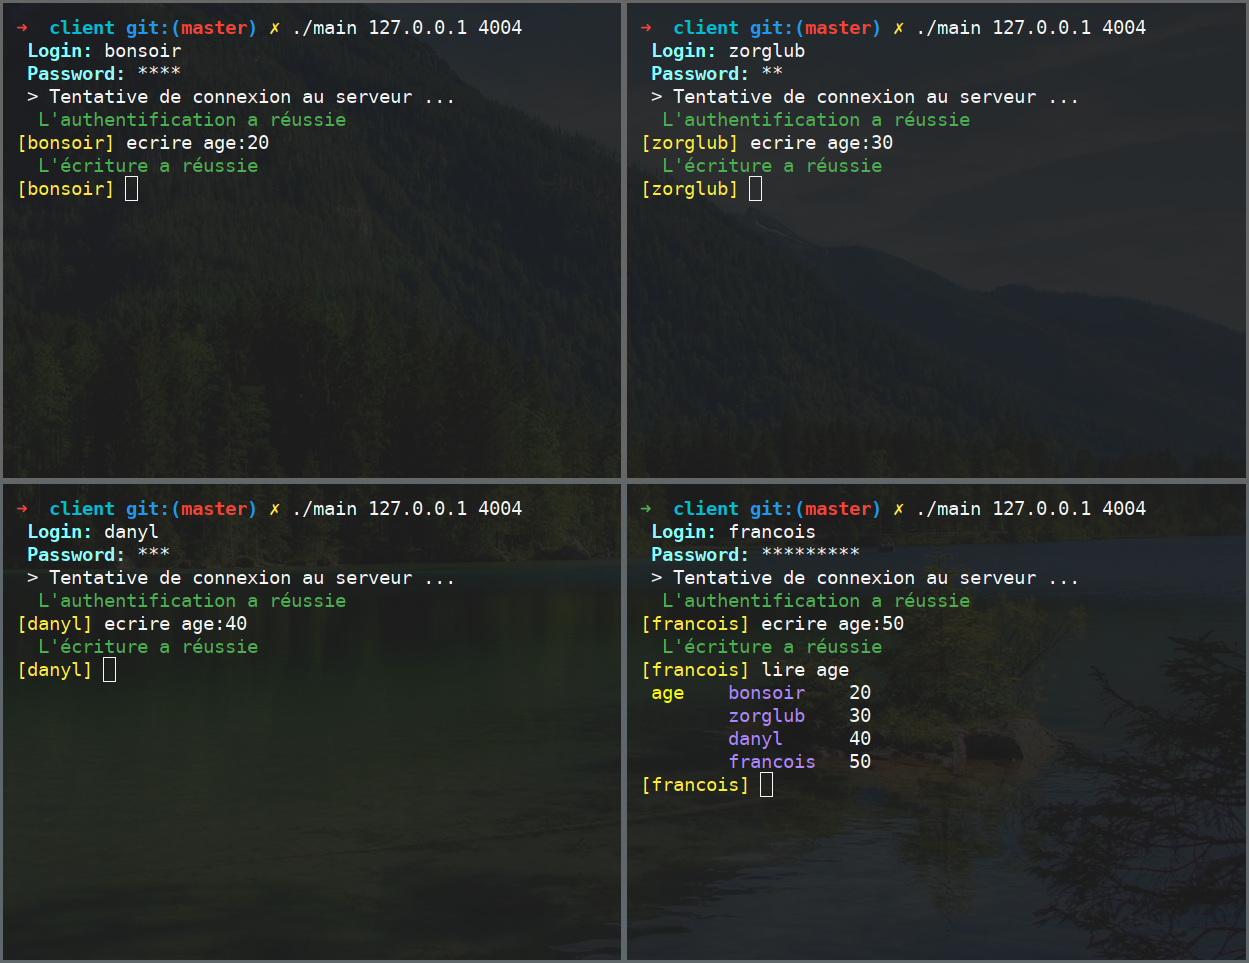
\includegraphics[scale=0.3]{img/testclients.png}
\end{center}

Le client a pour tâche principale de \textit{traduire les requêtes} de l'utilisateur (lecture, écriture, suppression, et autres) en requêtes pour le serveur d'accès.

Après une authentification réussie, l'utilisateur peut entrer les commandes suivantes:
\begin{itemize}
    \item \textbf{lire <champ[,\ldots]>}: obtenir les informations de tous les clients pour les champs demandés, si le client en a la permission.
    \item \textbf{écrire <champ1:valeur1[,\ldots]>}: modifier ses informations pour les champs demandés.
    \item \textbf{supprimer}: suppression de toutes ses informations.
    \item \textbf{aide}: afficher l'aide.
    \item \textbf{clear}: effacer l'écran actuel.
    \item \textbf{bye}: quitter proprement (prévenir le serveur d'accès de sa déconnexion, afin qu'il n'ai pas à attendre le timeout pour forcer la déconnexion).
\end{itemize}

Nous avons pris soin d'offrir une interface utilisateur simple et efficace à travers des petits "bonus" comme le masquage du mot de passe en astérisques, l'affichage d'un prompt, des couleurs, etc.

La déconnexion "propre" d'un client (bye) est également réalisée lors de la capture du signal \textbf{SIGINT}.

\subsection{Le serveur de données}

Le serveur de données doit traiter les requêtes du serveur d'accès et lui envoyer une réponse en fonction de ses données. Pour ce faire, il doit donc \underline{stocker une liste} associant un login à une valeur (donnée), ainsi que le champ qu'il doit gérer (âge, taille, etc.).

La méthode de connexion d'un serveur de données au serveur d'accès est la suivante:
\begin{enumerate}
    \item Le serveur de données envoie une requête \textbf{MEET} au serveur d'accès.
    \item Si le serveur d'accès lui répond, le serveur de données a bien été connecté.
    \item Si un serveur de données de \textit{même type} existait déjà dans le serveur d'accès, ce dernier va envoyer ses informations au nouveau afin de permettre une \textit{synchronisation permanente} des données au sein de la banque de données.
\end{enumerate}

Une fois connecté au serveur d'accès, le serveur de données peut donc recevoir ses requêtes et les traiter en lui envoyant une réponse. Lors de chaque message reçu, on vérifie que celui-ci \textit{provient bien du serveur d'accès} pour une question de \textbf{sécurité}.

\subsection{Les outils réseau (common)}

Les trois modules précédents partagent tous la même \textbf{API} réseau, qui a pour but de:
\begin{itemize}
    \item \textit{Unifier} l'envoi et la réception de données au bas niveau ainsi que d'autres utilitaires comme l'attente (sck.c).
    \item \textit{Fournir et automatiser} la "couche réseau" séparément de la couche principale des différents modules, afin qu'ils n'aient pas à gérer les mécanismes et problèmes susceptibles d'arriver lors des communications: il leur suffit d'appeler une fonction qui s'occupe de tout, par exemple:
    \begin{lstlisting}{language=c}
    int dgram_create_send (const int sck, dgram **dgsent, dgram **dgres, const uint16_t id,
                           const uint8_t request, const uint8_t status, const uint32_t addr,
                           const in_port_t port, const uint16_t data_size, const char *data);
    \end{lstlisting}
\end{itemize}

En utilisant cette API, les \textbf{principaux mécanismes} ci-dessous sont \textit{automatisés}:
\begin{itemize}
    \item Gestion des \textit{pertes}.
    \item \textit{Transformation} des données brutes en structures "dgram" (parser).
    \item Envoi d'un \textit{ACK} pour valider la réception d'un paquet.
    \item Assurer l'\textit{intégrité des données}.
    \item \textit{Ré envoi} des données si pas de ACK reçu après timeout.
    \item S'assurer que le message est "entier" (si non entier, attente des autres morceaux).
\end{itemize}

\newpage
Nous avons également pris soin d'implémenter un \textbf{système de débogage} en affichant les messages \textit{entrants} (IN) et \textit{sortants} (OUT) en affichant les données traduites en language humain des en-têtes et des données:

\begin{center}
    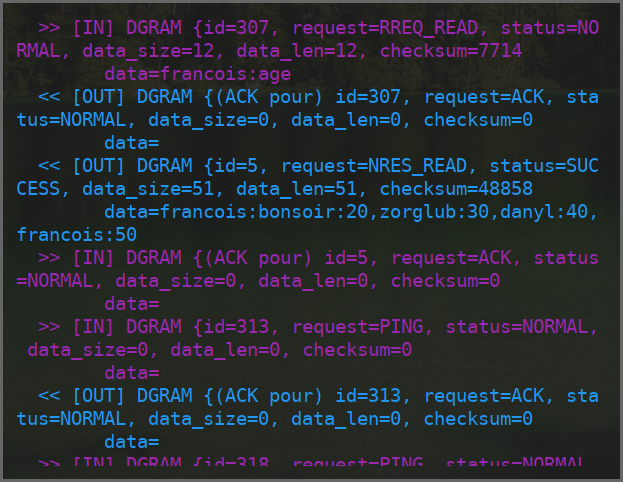
\includegraphics[scale=0.4]{img/debug.png}
\end{center}

\section{Protoles utilisés}

\subsection{Types de messages et status}

Nous avons choisis de séparer les \textit{types de messages} en 4 catégories:
\begin{enumerate}
    \item Client $\ra$ serveur d'accès (CREQ).
    \item Serveur d'accès $\ra$ serveur de données (RREQ et RNRES).
    \item Serveur de données $\ra$ serveur d'accès (NREQ et NRES).
    \item Serveur d'accès $\ra$ client (RRES).
\end{enumerate}

\begin{center}
    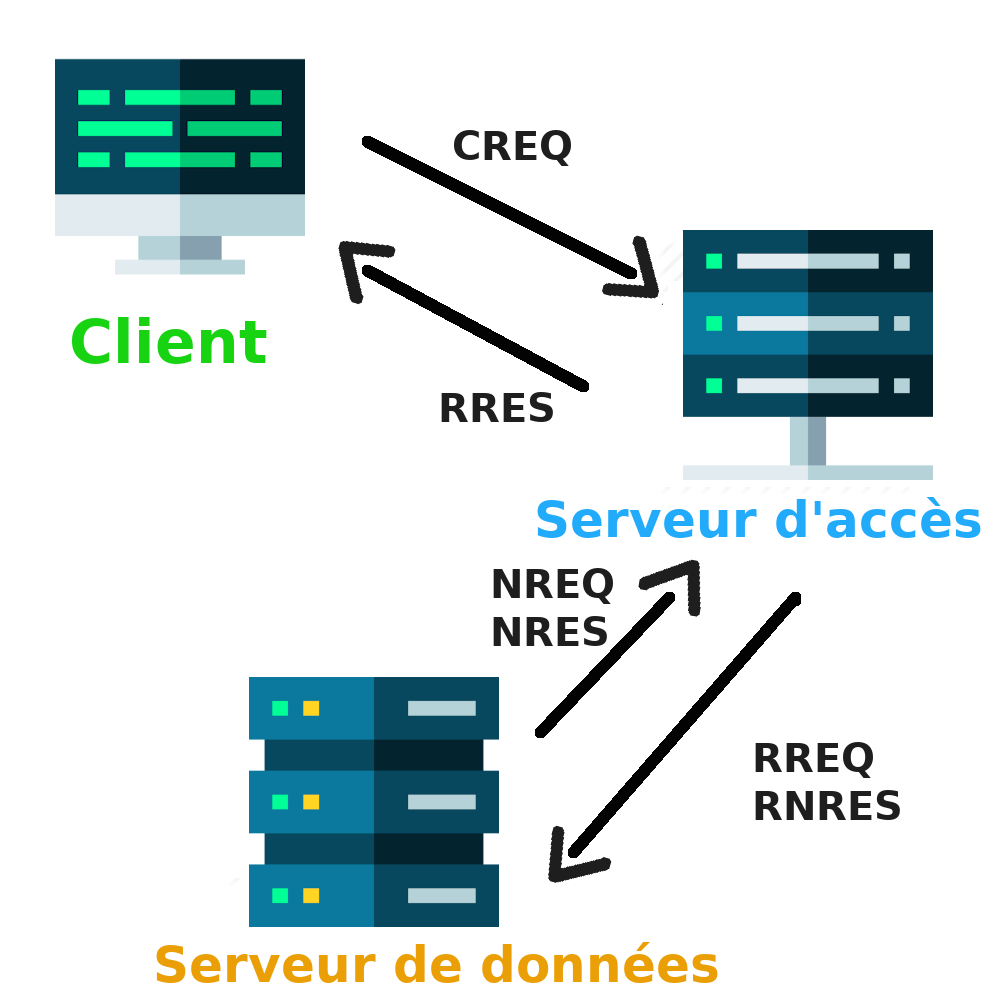
\includegraphics[scale=0.2]{img/req.png}
\end{center}

Ces préfixes sont suivis d'un type explicite de requête / réponse (AUTH, READ, WRITE, DELETE, MEET, GETDATA, SYNC, etc.).

\textit{MEET} permet la connecter un serveur de données au serveur d'accès.

\textit{GETDATA} permet de demander à un serveur de données qu'il envoie toutes ses données (pour futur SYNC).

\textit{SYNC} demander à un serveur de données de replacer toutes ses données par celles envoyées.

Le \textit{status} d'un message peut être:
\begin{itemize}
    \item SUCCESS $\ra$ succès de la requête (écriture réussie, etc.).
    \item NORMAL $\ra$ état normal (requête de lecture, etc.).
    \item ERR\_NOREPLY $\ra$ erreur, pas de réponse (le relais ne répond pas, etc.).
    \item ERR\_AUTHFAILED $\ra$ erreur, l'authentification a échouée.
    \item ERR\_NONODE $\ra$ erreur, aucun serveur de données correspondant trouvé.
    \item ERR\_NOPERM $\ra$ erreur, pas les permissions requises pour la lecture.
    \item ERR\_SYNTAX $\ra$ erreur de syntaxe.
    \item ETC
\end{itemize}

\subsection{Format des messages}

Chaque message qui transite entre un client, le serveur d'accès et un serveur de données contient \textbf{un en-tête} et les \textbf{données} elles-mêmes.

\begin{tabular}{|c|c|c|c|c|c|}
    \hline
    ID & Requête & Status & Taille données & Somme de contrôle & Données\\
    \hline
    16 bits & 8 bits & 8 bits & 16 bits & 16 bits & de 0 à 65536 octets\\
    \hline
\end{tabular}

\subsection{Structure de message et associés}

La structure qui représente un message (\textbf{dgram}) stocke, en plus des différentes attributs d'en tête et des données vues ci-dessus, divers éléments importants:
\begin{itemize}
    \item \textit{IP} et port de provenance / de destination.
    \item La \textit{date} de création / de réception (timestamp).
    \item Le nombre de ré envois (lorsque non réception de ACK de la part du récepteur du message).
    \item La \textit{fonction de callback} appelée lorsque le nombre de ré envois a enclenché le timeout associé, ainsi qu'un \textit{paramètre} pour ce callback.
\end{itemize}

Les \textit{fonctions associées} aux \textbf{dgram} nécessitent souvent une ou deux listes, qui sont propres à chaque module, parmi:
\begin{itemize}
    \item \underline{dgsent}: la liste des \textit{dgram envoyés}. Chaque message envoyé est \textbf{automatiquement supprimé} lors de la réception du ACK correspondant, ou après timeout. Les conserver permet de les \textit{ré envoyer} si le destinataire d'envoi pas de ACK de confirmation après un certain temps.
    \item \underline{dgreceived:} la liste des \textit{dgram reçus}. Chaque message reçu est automatiquement supprimé après envoi du ACK correspondant. Les conserver permet d'attendre que le message soit entier avant de l'utiliser (et timeout si non entier après un certain temps).
\end{itemize}

\subsection{Format des données}

Les messages ont un \textit{format bien précis} (en-tête + données), mais les données ont aussi un format précis qui varie selon qui est l'émetteur et qui est le récepteur entre le client, le serveur d'accès et le serveur de données. Connaître les formats utilisés (ci-dessous) ainsi que le format des messages, leur types et status permet l'\textit{interopérabilité} entre les modules développés ici et des modules externes dans le cas où tous utilisent les mêmes protocoles.

On suppose ici que les requêtes réussissent tous, et donc la section données n'est pas vide (sauf exceptions).

\subsubsection{Client $\ra$ Serveur d'accès (CREQ)}

\begin{itemize}
    \item \textit{Authentification:} <login>:<mot\_de\_passe>
    \item \textit{Lecture:} <champ>[,\ldots]
    \item \textit{Écriture:} <champ1>:<valeur1>[,\ldots]
    \item \textit{Suppression:} $\oslash$
    \item \textit{Bye:} $\oslash$
\end{itemize}

\subsubsection{Serveur d'accès $\ra$ Serveur de données (RREQ, RNRES)}

Dans le cas de RREQ (requête du serveur d'accès vers un serveur de données):
\begin{itemize}
    \item \textit{Lecture:} <login\_utilisateur>
    \item \textit{Écriture:} <login\_utilisateur>:<valeur>
    \item \textit{Suppression:} <login\_utilisateur>
    \item \textit{Synchronisation (SYNC):} <login1>:<valeur1>[,\ldots]
    \item \textit{Obtention données (GETDATA):} <id\_serveur\_donnée\_pour\_sync>
\end{itemize}

Dans le cas de RNRES (réponse du serveur d'accès à un serveur de données):
\begin{itemize}
    \item \textit{Rencontre (MEET):} $\oslash$
\end{itemize}

\subsubsection{Serveur de données $\ra$ Serveur d'accès (NREQ, NRES)}

Dans le cas de NREQ (requête du serveur de données vers le serveur d'accès):
\begin{itemize}
    \item \textit{Rencontre (MEET):} <champ>
\end{itemize}

Dans le cas de NRES (réponse du serveur de données au serveur d'accès):
\begin{itemize}
    \item \textit{Lecture:} <login1>:<valeur1>[,\ldots]
    \item \textit{Écriture:} $\oslash$
    \item \textit{Suppression:} $\oslash$
    \item \textit{Obtention données (GETDATA):} <id\_serveur\_données\_pour\_sync>:<login1>:<valeur1>[,<login2>:<valeur2>[,\ldots]]
\end{itemize}

\subsubsection{Serveur d'accès $\ra$ Client (RRES)}

\begin{itemize}
    \item \textit{Authentification:} $\oslash$
    \item \textit{Lecture:} <champ>:<login1>:<valeur1>[,<login2>:<valeur2>[,\ldots]]
    \item \textit{Écriture:} $\oslash$
    \item \textit{Suppression:} $\oslash$
    \item \textit{Bye:} $\oslash$
\end{itemize}

\section{Conclusion}

Réaliser ce projet n'a pas été des plus faciles (même le plus difficile jusqu'à présent, pour nous) mais nous a permis d'approfondir nos connaissances de la \textit{programmation sockets} et du \textit{réseau} en général et nous en sommes très content. Le développement de ce projet nous a également aidé à nous organiser pour le \textit{développement en collaboration} (Git).

\end{document}
